\begin{enumerate}[label=\thesubsection.\arabic*.,ref=\thesubsection.\theenumi]
\numberwithin{equation}{enumi} 
\item 
The asymptotic Bode magnitude plot of  minimum phase transfer function
G(s) is show below.
\begin{figure}[htp]
	\centering
	\includegraphics[width=1 \columnwidth]{./figs/ee18btech11009/pppp.eps}
	\caption{}
	\label{fig:given_bode}
\end{figure} 
%
Express $20\log\abs{G(j\omega)}$ as a function of $\omega$ using Fig \ref{fig:given_bode}.
\label{prob:plot} \\
\solution
\begin{align}
 20\log\abs{G(j\omega)} = 
 \begin{cases}
	60-20(\log(\omega)-\log(0.1)) \\   0.1 < \omega < 1 \\
	80-40(\log(\omega)-\log(0.1)) \\   1 < \omega < 20 \\
	126.02-60(\log(\omega)-\log(0.1)) \\   20 < \omega   
 \end{cases}
\end{align}


\item Express the slope of $20\log\abs{G(j\omega)}$ as a function of $\omega$. 
\\
\solution The desired slope is
\begin{align}
 \nabla20\log\abs{G(j\omega)} &= \dfrac{d(20\log\abs{G(j\omega)})}{d(\log(\omega))}
\end{align}
\begin{align}
 \nabla20\log\abs{G(j\omega)} = 
 \begin{cases}
	-20 &  \omega < 1 \\
	-40 & 1 < \omega < 20 \\
	-60 & 20 < \omega   
 \end{cases}
\end{align}

\item Express the change of slope of $20\log\abs{G(j\omega)}$ as a function of $\omega$. \\
\solution \\ 
 $\Delta(\nabla20\log\abs{G(j\omega)})$ = change of slope of $20\log\abs{G(j\omega)}$ at $\omega$ 
\begin{align}
 \Delta(\nabla20\log\abs{G(j\omega)}) = 
 \begin{cases}
    -20 &  \omega = 0 \\
	-20 &  \omega = 1 \\
	-20 &  \omega = 20
 \end{cases}
\end{align}

\item Find the poles and zeros of G(s).
\label{prob:bode} \\
\solution \\
Since, each pole corresponds to -20 dB/decade  
and each zero corresponds to +20 dB/decade.\\
there is a decrease in 20 dB/decade for each value of $\omega$ at 0,1,20.\\
$\therefore$ there exists \textbf{3 poles} and \textbf{no zeros}.

\item Find G(s) \\
\solution \\
From the solution of the problem \ref{prob:bode} we can obtain G(s)
\begin{align}
	G(s) = \frac{k}{s(1+s)(20+s)}
\end{align}

\item Obtain the Bode plot of G(s) through a python code and compare with the line plot of the expression that you obtained in Problem \ref{prob:plot} \\
\solution 
Fig \ref{fig:line_plot} shows the Bode plot of the transfer function obtained.\\
 The \textbf{Line plot} is the approximation of the \textbf{caluculated bode plot}. 
\begin{figure}[htp]
	\centering
	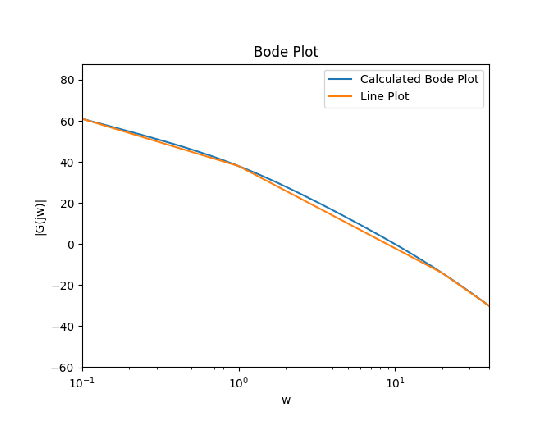
\includegraphics[width=1 \columnwidth]{./figs/ee18btech11009/plt.eps}
	\caption{}
	\label{fig:line_plot}
\end{figure} 


\item  Verify if at very high frequency $(\omega \to \infty)$, the phase angle $ \angle G(j\omega)=-3\pi/2$ \\
\solution \\
\textbf{Calculating phase:}\\ \\
Since we know that,\\
phase $ \phi $ is the sum of all the phases corresponding to each pole and zero.\\
phase corresponding to pole is =  
\begin{align}
-tan^{-1}( \frac{imaginary}{real})
\end{align} 
phase corresponding to zero is =
\begin{align}
 tan^{-1}( \frac{imaginary}{real})
 \end{align} 
%------------------------------------------------
Now take,
\begin{align}
 s = j\omega
  \end{align} 
  \begin{align}
 \Rightarrow  G(j\omega) =  \frac{k}{j\omega(1+j\omega)(20+j\omega)}
 \end{align} 
Therefore, 
\begin{align}
 \phi =  -tan^{-1}( {\frac{\omega}{0}}) - tan^{-1}(\omega) - tan^{-1}( \frac{\omega}{20})
 \end{align} 
 \begin{align}
  \phi =  - 90^\circ - tan^{-1}(\omega) - tan^{-1}( \frac{\omega}{20})
  \end{align} 
  \begin{align}
  \because \omega \to \infty
 \end{align} 
 \begin{align}
   \phi =   - 90^\circ - 90^\circ - 90^\circ
   \end{align} 
   \begin{align}
 \phi = -270^\circ
 \end{align} 
 \begin{align}
 \phi = -3\pi/2 
 \end{align} 
 $\therefore$ at very high frequency $(\omega \to \infty)$, the phase angle $ \angle G(j\omega)=-3\pi/2$.
 \item

\end{enumerate}
